%%%%%%%%%%%%%%%%%%%%%%%VICARIOUS%%%%%%%%%%%%%%%%%%%%%%%%%%%%%%%%%%%%%%%
% Copyright ME, FUCK YOU												%
% Template for presentation in Latex`s Beamer Class					%
% Using the default Berlin theme, can be replaced by other themes		%
% logo in the upper right can be replaced by new .png, gif, eps etc	%
% 																		%
%%%%%%%%%%%%%%%%%%%%%%%%%%%%%%%%%%%%%%%%%%%%%%%%%%%%%%%%%%%%%%%%%%%%%%%
\documentclass[xcolor=dvipsnames]{beamer}
\usetheme{Berlin}
\usecolortheme[named=LimeGreen]{structure}
\usepackage{beamerthemesplit} % kam neu dazu
\usepackage[ngerman]	{babel}			
\usepackage{t1enc}						
\usepackage[utf8]{inputenc}			
\usepackage{amsmath}
\usepackage{graphicx}
\graphicspath{{pictures/}}
\usepackage{amssymb}
\usepackage{amsfonts}
\usepackage{caption}
\usepackage{multimedia}
\usepackage{tikz}
\usepackage{listings}
\usepackage{acronym}

\usepackage{lmodern}
\usepackage{multicol}


\definecolor{pblue}{rgb}{0.13,0.13,1}
\definecolor{pgreen}{rgb}{0,0.5,0}
\definecolor{pred}{rgb}{0.9,0,0}
\definecolor{pgrey}{rgb}{0.46,0.45,0.48}

\lstset{
    escapeinside={(*}{*)}
}

\lstdefinestyle{Java}{
  showspaces=false,
  showtabs=false,
  tabsize=2,
  breaklines=true,
  showstringspaces=false,
  breakatwhitespace=true,
  commentstyle=\color{pgreen},
  keywordstyle=\color{pblue},
  stringstyle=\color{pred},
  basicstyle=\footnotesize\ttfamily,
  numbers=left,
  numberstyle=\tiny\color{gray}\ttfamily,
  numbersep=7pt,
  %moredelim=[il][\textcolor{pgrey}]{$$},
  moredelim=[is][\textcolor{pgrey}]{\%\%}{\%\%},
  captionpos=b
}

\lstdefinestyle{basic}{  
  basicstyle=\footnotesize\ttfamily,
  breaklines=true
  numbers=left,
  numberstyle=\tiny\color{gray}\ttfamily,
  numbersep=7pt,
  backgroundcolor=\color{white},
  showspaces=false,
  showstringspaces=false,
  showtabs=false,
  frame=single,
  rulecolor=\color{black},
  captionpos=b,
  keywordstyle=\color{blue}\bf,
  commentstyle=\color{gray},
  stringstyle=\color{green},
  keywordstyle={[2]\color{red}\bf},
}


\lstdefinelanguage{custom}
{
morekeywords={public, void},
sensitive=false,
morecomment=[l]{//},
morecomment=[s]{/*}{*/},
morestring=[b]",
}


\lstdefinestyle{BashInputStyle}{
  language=bash,
  showstringspaces=false,
  basicstyle=\small\sffamily,
  numbers=left,
  numberstyle=\tiny,
  numbersep=5pt,
  frame=trlb,
  columns=fullflexible,
  backgroundcolor=\color{gray!20},
  linewidth=0.9\linewidth,
  xleftmargin=0.1\linewidth
}

%Logo in the upper right just change if you know what you are doing^^
\addtobeamertemplate{frametitle}{}{%
\begin{tikzpicture}[remember picture,overlay]
\node[anchor=north east,yshift=2pt] at (current page.north east) {
\includegraphics[height=1.8cm]{htw}};
\end{tikzpicture}}

\begin{document}
\bibliographystyle{alpha}
\title{Netzwerke -- Seminaristische Übung WS17/18}
\subtitle{Bit-Arithmetik \& OSI Layer III\\
		\href{mailto:Benjamin.Troester@HTW-Berlin.de}{Benjamin.Troester@HTW-Berlin.de}\\
		PGP: ADE1 3997 3D5D B25D 3F8F 0A51 A03A 3A24 978D D673 }
\author{Benjamin Tröster}

\date{\today}

\begin{frame}
\titlepage
\end{frame}

\section*{Road-Map}
\begin{frame}
\frametitle{Road-Map}
\begin{multicols}{2}
  \tableofcontents
\end{multicols}
\end{frame}

\section*{Stuff}
\begin{frame}{Nerd-Wochenmarkt}
Empfehlung der Woche:
\begin{itemize}
	\item CRE: Technik, Kultur, Gesellschaft ist ein unregelmäßig erscheinender Interview-Podcast.
	\begin{itemize}
		\item IPv4: \url{https://cre.fm/cre141-ipv4} 
	\end{itemize}
	\item Pentaradio24 ist ein Podcast des C3D2
	\begin{itemize}
		\item Raspberry Pi: \url{https://c3d2.de/news/pentaradio24-20130122.html} 
	\end{itemize}
\end{itemize}
\end{frame}

\begin{frame}{Retrospektive}
\begin{itemize}
	\item Vorlesung
	\begin{itemize}
		\item Fragen?
	\end{itemize}
	\item Übungsblatt
	\begin{itemize}
		\item Auflösung des letzten Aufgabenblatts
		\item Fragen?
	\end{itemize}
\end{itemize}
\end{frame}

\section{Raspberry Pi}
\begin{frame}
 \hspace*{-1cm}
\begin{minipage}{0.7\textwidth}
\begin{itemize}
	\item Raspberry Pi 1+ Model B -- System on a Chip (SoC)
	\item Architektur: ARMv6Z (32-bit)
	\item  ARM11 -- 700 MHz @ 1 Core
	\item 512 MB RAM
	\item 10/100 Mbit/s Ethernet (8P8C)
	\item HDMI (rev 1.3),
	\item Raspbian 9 Stretch -- Debian Fork
\end{itemize}
\end{minipage}%
\begin{minipage}{0.3\textwidth}
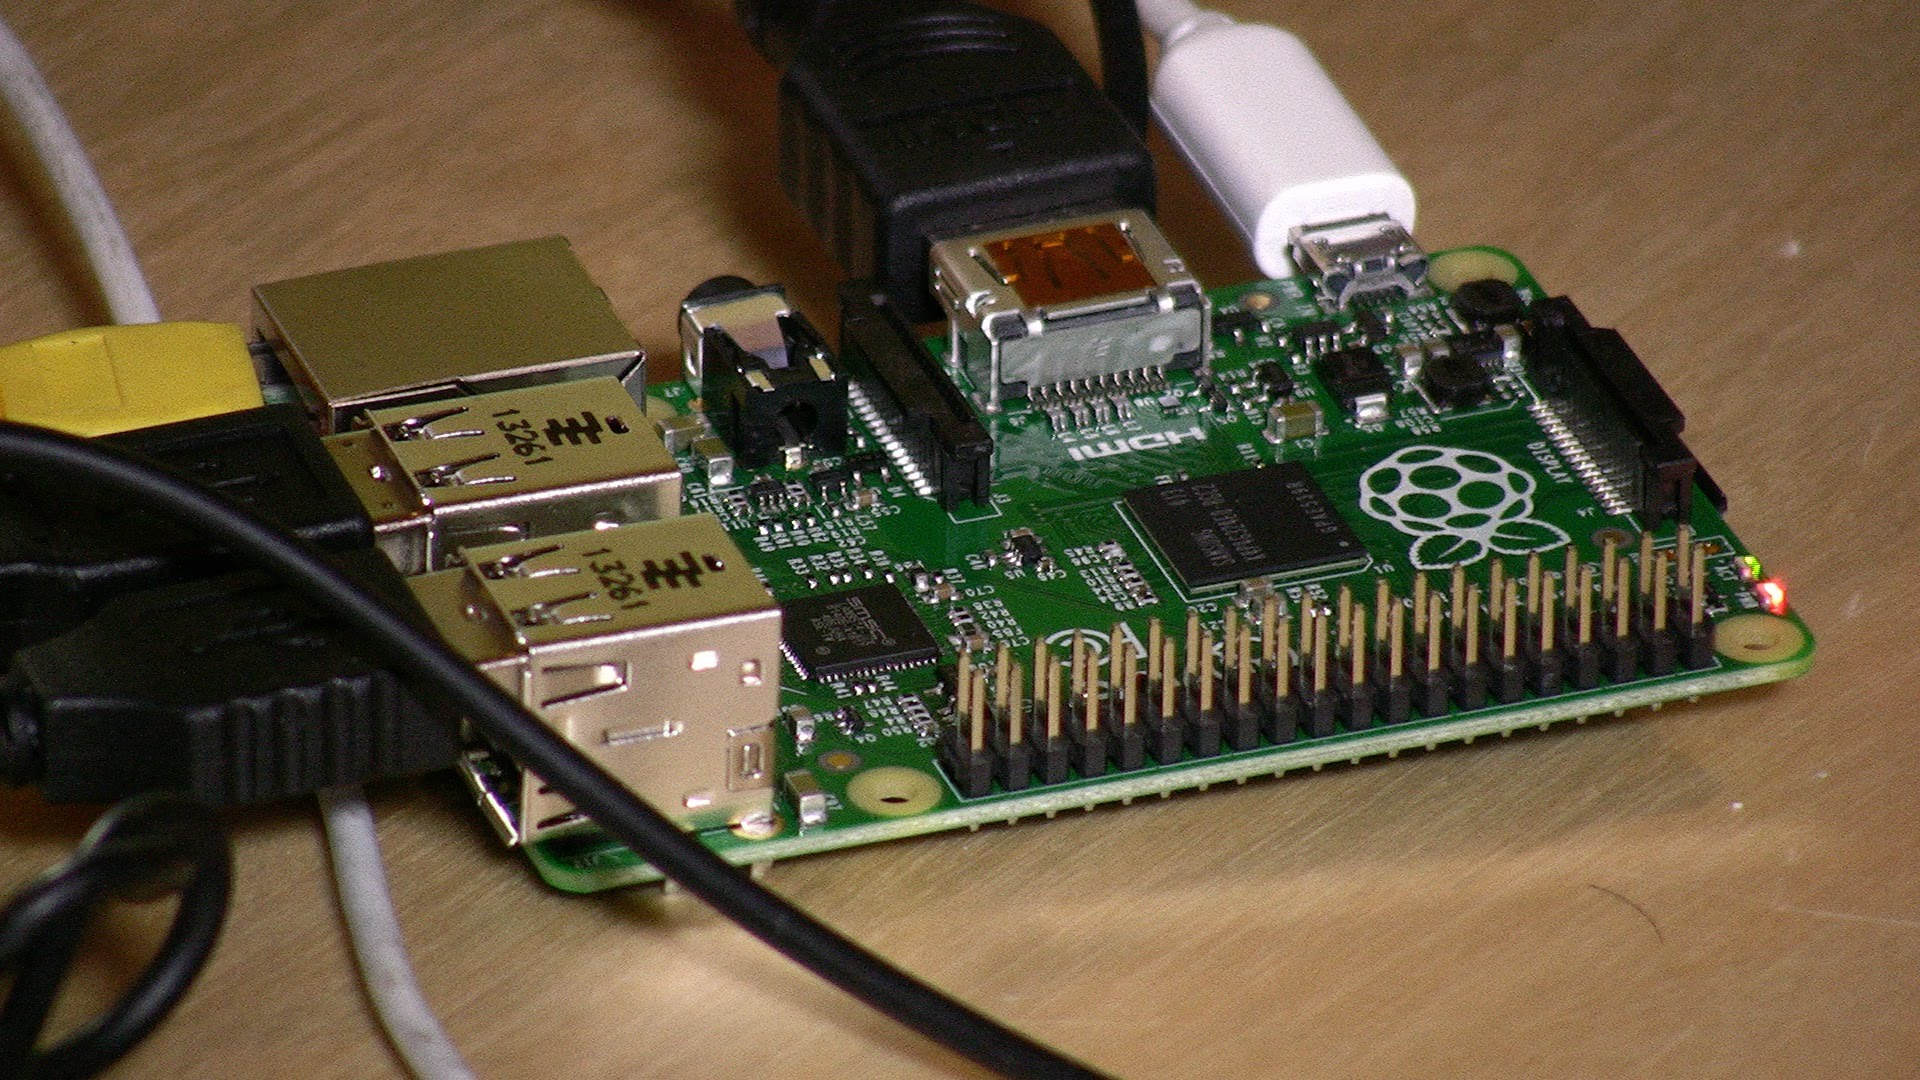
\includegraphics[scale=0.07]{raspi}
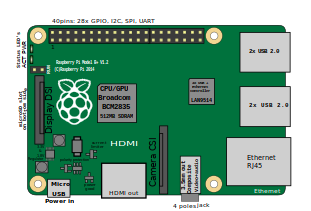
\includegraphics[scale=0.45]{raspib1+}
\end{minipage}\hfill
\end{frame}

\section{Übung}
\begin{frame}
\begin{itemize}
	\item Heute erste Hands-On-Übung!
	\item Wir bauen ein kleines Netzwerk auf
	\item Theorieaufgaben liegen im Moodle
\end{itemize}
\end{frame}

\end{document}